% Options for packages loaded elsewhere
\PassOptionsToPackage{unicode}{hyperref}
\PassOptionsToPackage{hyphens}{url}
%
\documentclass[
  12pt,
]{article}
\usepackage{amsmath,amssymb}
\usepackage{iftex}
\ifPDFTeX
  \usepackage[T1]{fontenc}
  \usepackage[utf8]{inputenc}
  \usepackage{textcomp} % provide euro and other symbols
\else % if luatex or xetex
  \usepackage{unicode-math} % this also loads fontspec
  \defaultfontfeatures{Scale=MatchLowercase}
  \defaultfontfeatures[\rmfamily]{Ligatures=TeX,Scale=1}
\fi
\usepackage{lmodern}
\ifPDFTeX\else
  % xetex/luatex font selection
\fi
% Use upquote if available, for straight quotes in verbatim environments
\IfFileExists{upquote.sty}{\usepackage{upquote}}{}
\IfFileExists{microtype.sty}{% use microtype if available
  \usepackage[]{microtype}
  \UseMicrotypeSet[protrusion]{basicmath} % disable protrusion for tt fonts
}{}
\makeatletter
\@ifundefined{KOMAClassName}{% if non-KOMA class
  \IfFileExists{parskip.sty}{%
    \usepackage{parskip}
  }{% else
    \setlength{\parindent}{0pt}
    \setlength{\parskip}{6pt plus 2pt minus 1pt}}
}{% if KOMA class
  \KOMAoptions{parskip=half}}
\makeatother
\usepackage{xcolor}
\usepackage[left=3.5cm,right=1cm,top=3cm,bottom=1.5cm]{geometry}
\usepackage{graphicx}
\makeatletter
\def\maxwidth{\ifdim\Gin@nat@width>\linewidth\linewidth\else\Gin@nat@width\fi}
\def\maxheight{\ifdim\Gin@nat@height>\textheight\textheight\else\Gin@nat@height\fi}
\makeatother
% Scale images if necessary, so that they will not overflow the page
% margins by default, and it is still possible to overwrite the defaults
% using explicit options in \includegraphics[width, height, ...]{}
\setkeys{Gin}{width=\maxwidth,height=\maxheight,keepaspectratio}
% Set default figure placement to htbp
\makeatletter
\def\fps@figure{htbp}
\makeatother
\setlength{\emergencystretch}{3em} % prevent overfull lines
\providecommand{\tightlist}{%
  \setlength{\itemsep}{0pt}\setlength{\parskip}{0pt}}
\setcounter{secnumdepth}{5}
\ifLuaTeX
\usepackage[bidi=basic]{babel}
\else
\usepackage[bidi=default]{babel}
\fi
\babelprovide[main,import]{spanish}
% get rid of language-specific shorthands (see #6817):
\let\LanguageShortHands\languageshorthands
\def\languageshorthands#1{}
\renewcommand{\contentsname}{Contenido}
\usepackage{setspace}
\doublespacing

\usepackage{float}
\usepackage{caption}
\usepackage{xcolor}
\usepackage{geometry}

\captionsetup{
  font={bf,small},
  labelfont={bf},
  justification=centering,
  position=top,
  singlelinecheck=false
}

\captionsetup[table]{
  position=top,
  skip=5pt
}

\captionsetup[figure]{
  position=above,
  skip=5pt
}
\usepackage{booktabs}
\usepackage{longtable}
\usepackage{array}
\usepackage{multirow}
\usepackage{wrapfig}
\usepackage{float}
\usepackage{colortbl}
\usepackage{pdflscape}
\usepackage{tabu}
\usepackage{threeparttable}
\usepackage{threeparttablex}
\usepackage[normalem]{ulem}
\usepackage{makecell}
\usepackage{xcolor}
\ifLuaTeX
  \usepackage{selnolig}  % disable illegal ligatures
\fi
\usepackage{bookmark}
\IfFileExists{xurl.sty}{\usepackage{xurl}}{} % add URL line breaks if available
\urlstyle{same}
\hypersetup{
  pdflang={es},
  hidelinks,
  pdfcreator={LaTeX via pandoc}}

\author{}
\date{\vspace{-2.5em}}

\begin{document}

\newgeometry{left=2.5cm, right=2.5cm, top=2.5cm, bottom=2.5cm}
\begin{titlepage}
\centering

% --- Título del proyecto ---
{\Huge \textbf{Métrica RAPM: Evaluación del impacto ofensivo y defensivo de los jugadores de la Liga Nacional de Básquetbol en Argentina}\par}

\vspace{1.5cm}

% --- Subtítulo ---
{\LARGE \textbf{Tesina de grado}\par}

\vspace{2cm}

% --- Datos del autor y directores ---
{\Large Estudiante: Simón Pedro Gazze\par}
{\Large Director: Andrés Sosa\par}
{\Large Co-directora: Cristina Cuesta\par}

\vspace{2cm}

% --- Fecha ---
{\Large Fecha: 18 de febrero de 2026\par}

\vfill

% --- Logo centrado ---
\includegraphics[height=2.8cm]{Logo-unr.png}  % Cambiá por unr.png si corresponde

\end{titlepage}

\pagebreak

\restoregeometry

\newpage

\renewcommand{\contentsname}{Contenido}
\tableofcontents
\newpage

\section{Resumen}\label{resumen}

El crecimiento de la analítica deportiva ha impulsado el desarrollo de
métricas destinadas a evaluar con mayor precisión la contribución de los
jugadores al rendimiento de sus equipos. Particularmente en el
básquetbol, las estadísticas individuales derivadas del box score
presentan limitaciones para capturar el impacto real de los jugadores
sobre el resultado del juego. Una de las medidas desarrolladas con este
propósito es el \emph{plus-minus}, que registra la diferencia de puntos
generada mientras un jugador permanece en cancha. Sin embargo, esta
métrica presenta dificultades para aislar el efecto propio de cada
jugador respecto del contexto en el que participa. En respuesta a esta
problemática surge el \emph{Regularized Adjusted Plus Minus}
(\emph{RAPM}), una medida basada en modelos estadísticos que estima el
impacto ofensivo y defensivo de cada jugador controlando simultáneamente
la presencia de compañeros y rivales en cancha.

El objetivo de este trabajo es estimar el impacto individual de los
jugadores de la Liga Nacional de Básquetbol de Argentina durante la
temporada 2024/2025 mediante modelos RAPM, construyendo rankings que
permitan identificar y comparar sus contribuciones ofensivas y
defensivas. Asimismo, se analizan distintas alternativas metodológicas
para abordar problemas recurrentes en este tipo de modelos,
particularmente la multicolinealidad entre jugadores y la presencia de
coeficientes extremos asociados a jugadores con escasa participación en
cancha.

, las acciones registradas fueron agrupadas en posesiones, que
constituyen la unidad de análisis utilizada para la estimación de las
métricas propuestas. Inicialmente, se ajustaron modelos de regresión
lineal múltiple, incorporando distintas técnicas de regularización.
Posteriormente, se implementaron modelos de regresión logística
multinomial que representan de manera más adecuada la naturaleza
discreta de la variable respuesta. A partir de las probabilidades
estimadas por estos modelos se construyeron métricas basadas en puntos
esperados por posesión (\emph{EPTS}). Finalmente, se propuso una
ponderación a dicha métrica denominada \emph{wEPTS}, que incorpora la
participación de cada jugador relativa a las posesiones de su equipo con
el objetivo de penalizar a los jugadores con poco tiempo de juego. Los
resultados obtenidos muestran que esta métrica presentó un desempeño
superior al de las alternativas propuestas, de acuerdo con los distintos
criterios de validación utilizados.

Este estudio constituye la primera aplicación de métricas \emph{RAPM} en
la Liga Nacional de Básquetbol de Argentina y aporta una metodología
reproducible para la evaluación objetiva del rendimiento individual de
los jugadores, contribuyendo al desarrollo de herramientas de analítica
deportiva en el contexto del básquetbol argentino.

\textbf{Palabras clave}: básquetbol, analítica en el deporte, Liga
Nacional de Básquet, plus-minus, RAPM, regresión logística multinomial,
regularización.

\newpage

\section{Introducción}\label{introducciuxf3n}

\subsection{Sports Analytics}\label{sports-analytics}

\emph{Sports Analytics} o analítica en el deporte es un término que
refiere a la aplicación de métodos estadísticos para describir, explicar
y/o predecir fenómenos vinculados al rendimiento deportivo, tanto a
nivel individual como colectivo con el objetivo de facilitar la toma de
decisiones de entrenadores o \emph{staff} técnico antes, durante y
después de los partidos.

A pesar de que las primeras aplicaciones al análisis de datos al deporte
se remontan a mediados del siglo XX, el impulso más significativo
ocurrió a partir del año 2000, en particular en el béisbol, con la
popularización del enfoque conocido como \emph{sabermetrics}\footnote{Término
  utilizado para referirse al análisis estadístico del béisbol, basado
  en la recopilación y estudio sistemático de datos con el fin de
  comprender y cuantificar el desempeño de los jugadores y equipos. El
  nombre proviene de SABR (\emph{Society for American Baseball
  Research}).}. Desde entonces, la práctica se extendió a otros deportes
como el básquetbol, el fútbol o el tenis; dando lugar a una nueva
cultura de toma de decisiones basada en evidencia. Hoy en día, los
equipos profesionales, las ligas y las federaciones emplean
departamentos especializados en análisis de datos para optimizar
estrategias de juego, evaluar el rendimiento de jugadores, prevenir
lesiones y gestionar recursos económicos de manera más eficiente.

El \textbf{básquetbol} es uno de los deportes que más ha incorporado el
análisis estadístico en su evolución reciente. Desde las primeras
métricas derivadas del \emph{box score} (resumen estructurado de los
resultados de un partido), el desarrollo de bases de datos
\emph{play-by-play} (registro de cada una de las acciones del partido) a
partir de la década del 2000 hasta la incorporación más reciente de
tecnologías de \emph{player tracking} (sistema que utiliza cámaras y
software de visión artificial en los estadios para registrar los
movimientos de jugadores y pelotas en tiempo real). A partir de esta
información, se han desarrollado distintas herramientas estadísticas
para poder estudiar la eficiencia de los jugadores, la eficiencia de los
lanzamientos al aro, el desempeño de los equipos, la importancia en la
creación de espacios, entre otras cosas.

\subsection{Medidas de desempeño para jugadores de
básquetbol}\label{medidas-de-desempeuxf1o-para-jugadores-de-buxe1squetbol}

Desde la consolidación del \emph{box-score} en el básquetbol
profesional, durante la década de 1950, empezaron a calcularse las
primeras medidas de desempeño para los jugadores, como pueden ser los
puntos, rebotes, asistencias, etc. Durante mucho tiempo estas métricas
constituyeron una de las formas más tradicionales de evaluar el
rendimiento individual en el básquetbol. Su amplia disponibilidad y
fácil interpretación las convirtieron en el principal insumo para
comparar jugadores, otorgar premios o negociar contratos. Estas medidas
suelen agruparse en un conjunto de estadísticas denominadas
\emph{bottom-up}, las cuales se calculan en función de las acciones
individuales de los jugadores, es decir, si un jugador realiza una
acción que se asocia con un resultado positivo para el equipo, la
calificación de ese jugador aumenta, mientras que la calificación de los
demás jugadores, que no participaron en la jugada, permanece sin
cambios. Pero estas medidas presentan algunas limitaciones importantes,
ya que, sólo capturan una parte de los eventos relevantes del partido
(acciones como una defensa asfixiante, buenas rotaciones defensivas o
pases rápidos para iniciar una posesión no están contempladas) y no
necesariamente reflejan el impacto real de un jugador en las victorias
de su equipo, que es lo que importa a fin de cuentas.

Por otra parte, las medidas \emph{top-down} se basan en el rendimiento
del equipo en su conjunto, y el crédito por dicho rendimiento se
distribuye entre los jugadores que estuvieron involucrados en el
partido, sin importar qué acciones puntuales hayan realizado.

Con la idea de que lo más importante en un partido es \textbf{ganar}, y
entendiendo que las estadísticas tradicionales son solo una medida
imperfecta de muchas de las contribuciones que realizan los jugadores a
la victoria, en este trabajo buscaremos ``pensar más allá del \emph{box
score}'' y nos centraremos en estadísticas \emph{top-down}, más
precisamente en la medida \emph{Plus/Minus}. Esta estadística registra
los cambios que se producen en el marcador durante los minutos en que el
jugador de interés está en cancha, partiendo de la idea de que los
equipos deberían rendir mejor (reflejado en un \emph{Plus/Minus} más
alto) cuando sus buenos jugadores están en cancha que cuando no lo
están. Sin embargo esta métrica posee una deficiencia clave: \textbf{la
calificación de cada jugador va a depender en gran medida de la calidad
de sus compañeros en el campo}. Por ejemplo: un jugador de rol dentro de
un gran equipo va a tener un mayor \emph{Plus/Minus} que una
superestrella en un equipo con mal desempeño.

\subsection{RAPM (Regularized Adjusted Plus
Minus)}\label{rapm-regularized-adjusted-plus-minus}

La deficiencia anteriormente mencionada se ha intentado solucionar
implementando \textbf{modelos matemáticos} que incorporen los efectos
tanto de los compañeros presentes en cancha como de los rivales en ese
momento, buscando aislar el efecto real de los jugadores en la cancha.
El primero en realizar una publicación sobre el tema fue Dan Rosenbaum
(2004), el cual planteó un \textbf{modelo de regresión lineal múltiple}
en base a observaciones provenientes de partidos de las temporadas
2002-2003 y 2003-2004 de la National Basketball Association o
\emph{NBA}. Como unidad de análisis se utilizaron segmentos de partidos
donde no ocurrian sustituciones, la variable respuesta fue la diferencia
en el marcador entre el equipo local y el visitante en ese segmento; y
como variables explicativas se postularon variables dicotómicas para
cada uno de los jugadores que hayan jugado al menos un partido en esas
temporadas. Finalmente las métricas de desempeño se correspondían con
los coeficientes estimados que acompañaban a las ``Dummies'' de cada
jugador, dichas estimaciones se realizaron mediante la técnica de
Mínimos Cuadrados Ordinarios. Estas estadísticas se conocen como
\emph{Adjusted Plus Minus} (APM).

A pesar de que estas métricas presentaban una solución innovadora a la
problematica inicial, Rosenbaum señaló que las estimaciones obtenidas no
resultaron muy precisas. El modelo propuesto presentaba estimaciones con
mucho error, debido a un claro problema de \textbf{multicolinealidad} ya
que muchos de los jugadores compartían una gran cantidad de minutos
juntos en cancha, y se necesitaba de una gran cantidad observaciones de
varias temporadas para que el modelo pudiera separar el efecto propio de
cada jugador.

Para solucionar está problemática, se plantea la métrica RAPM
introducida por Sill (2010) en la cual se aborda el problema de la
Multicolinealidad mediante estimaciones de los parametros realizadas con
Métodos de Regularización, particularmente utilizando la
\textbf{Regresión Ridge}. Esté método de regularización es el más
abordado a lo largo de toda la literatura relevante sobre RAPM hasta la
fecha.

Otro de los problemas recurrentes en estos modelos esta relacionado con
la inclusión de jugadores que participan muy pocos minutos en cancha
(\emph{LTPs - Low time Players}). Cuando un jugador juega muy poco, el
modelo solo tiene unas pocas observaciones (segmentos) para evaluarlo, y
si particularmente en esas observaciones el equipo tiene un muy buen
desempeño (probablemente por casualidad); entonces el modelo no puede
diferenciar si el efecto es propio del jugador y estima coeficientes
extremos. Para solucionar estos casos se han contemplado las siguientes
alternativas: 1) excluir a los jugadores con pocos minutos dentro de las
temporadas (por ejemplo: Rosembaum (2004) excluye a lo jugadores con
menos de 250 minutos, Ilardi (2007) excluyen a lo jugadores con menos de
400 minutos, etc), 2) utilizar una gran cantidad de observaciones
(Ilardi \& Barzilai (2008) incorpora información de 5 temporadas), 3)
plantear métodos de estimación de los parámetros que penalicen a este
tipo de jugadores.

En los últimos años, muchos investigadores han publicado trabajos
orientados a mejorar los resultados de las métricas RAPM.
Particularmente en este trabajo se usa como referencia central al
artículo titulado: \textbf{Lasso multinomial performance indicators for
in‑play basketball data (Damoulaki et.al , 2025)}, el cual presenta
diferencias importantes respecto de los estudios previos. Dicho artículo
utiliza \textbf{posesiones} (definidas, según Kubatko et al.~(2007),
como el periodo que comienza cuando un equipo obtiene el control de la
pelota y termina cuando cede su control al rival) como unidad de
análisis, \textbf{puntos} en esas posesiones como variable respuesta y
emplea \textbf{modelos logísticos multinomiales} que representan de
manera más adecuada la naturaleza de la respuesta.

\section{Motivación}\label{motivaciuxf3n}

El creciente interés por la analítica deportiva que se ha evidenciado en
los últimos años en distintos paises del mundo, ha empezado a captar la
atención de las entidades deportivas en Argentina. Particularmente este
año la Confederación Argentina de Básquetbol (CABB) y la Asociación de
Clubes (AdC) anunciaron en octubre la ampliación de su alianza con
Catapult (empresa australiana de tecnología deportiva), integrando
equipamiento de \emph{wearables} (GPS) y software de videoanálisis para
las 19 franquicias de la Liga Nacional, las 34 de la Liga Argentina y
las selecciones nacionales en todas las ramas. Mientras que en el ámbito
educativo, el Instituto CAB (creado en 2023) realizó un convenio con
Sports Data Campus (España) para ofrecer, en agosto de este año, el
primer curso de \emph{Big Data aplicado al básquetbol} en Argentina, con
el objetivo de que entrenadores y \emph{staff} técnico colaboren en
proyectos reales de la CABB, aportando soluciones basadas en datos sobre
rendimiento, \emph{scouting} y optimización de procesos\footnote{Confederación
  Argentina de Básquetbol (2025). \emph{La Confederación Argentina de
  Básquet y Sports Data Campus firman un acuerdo de colaboración}.
  \href{https://www.argentina.basketball/ver/noticia/la-confederacion-argentina-de-basquet-y-sports-data-campus-firman-un-acuerdo-de-colaboracion}{Link
  al artículo}.}.

Estas cuestiones previamente mencionadas dan indicio de que estamos ante
un momento ideal para profundizar en el estudio y la aplicación del
análisis de datos en el básquetbol. Se trata de un área que comienza a
reconocerse como un componente fundamental tanto para mejorar el
rendimiento deportivo de los equipos como para impulsar el desarrollo
del negocio en torno al deporte. Sin embargo, el potencial de la
analítica aplicada al básquetbol en Argentina aún pareciera encontrarse
lejos de estar plenamente aprovechado.

En este marco, y con el fin de caracterizar el estado de situación del
análisis de datos en el básquet argentino, se relevaron los proyectos e
iniciativas actualmente activos en el país vinculados a la estadística y
la tecnología aplicada al deporte.

\begin{itemize}
\item
  \emph{CHAS All Stats}, dirigido por Facundo Salas y Sebastián Fiol,
  ambos entrenadores de básquetbol Nivel 3 Eneba, especialistas en
  estadísticas avanzadas y analistas de datos en equipos profesionales.
  Ofrecen servicios de análisis táctico y brindan cursos de estadísticas
  avanzadas.
\item
  \emph{Básquet Advance}, dirigido por el entrenador Cristian Sánchez,
  ofrece informes pre/post partido con estadísticas avanzadas y
  tendencias clave para entrenadores y scouts.
\end{itemize}

Ambos proyectos ofrecen herramientas muy importantes y de gran valor
tanto para los equipos como para el desarrollo del análisis de datos en
el deporte. Pero particularmente en ambos casos, los que llevan adelante
estos proyectos son entrenadores de básquetbol, los cuales a pesar de
que pueden contar con una sólida formación técnica, no son profesionales
de ciencias estadística o matemática.

Por este motivo, resulta fundamental la incorporación de profesionales
en carreras de ciencias exactas, que trabajen en conjunto con los
entrenadores y cuerpos técnicos, para de esta manera poder ofrecer
nuevos análisis más rigurosos y profundos, así como mejorar las
herramientas actualmente disponibles. Esta correspondencia entre el
conocimiento técnico-deportivo y el enfoque estadístico permitiría
potenciar el desarrollo del básquet argentino y contribuir a elevar su
nivel competitivo en un futuro.

\newpage

\section{Objetivos}\label{objetivos}

\subsection{Objetivo general}\label{objetivo-general}

El objetivo general de esta tesina es estimar el aporte individual de
los jugadores de la Liga Nacional de Básquetbol de Argentina durante la
temporada 2024/2025 mediante modelos RAPM, con el fin de construir un
ranking que refleje su impacto en el desempeño de sus equipos.

\subsection{Objetivos específicos}\label{objetivos-especuxedficos}

\begin{enumerate}
\def\labelenumi{\arabic{enumi})}
\item
  Generar una base de datos del tipo \emph{play-by-play} para la
  temporada 2024/2025 de la Liga Nacional de Básquetbol de Argentina,
  mediante técnicas de \emph{web scraping}.
\item
  Diferenciar el aporte ofensivo y defensivo de cada uno de los
  jugadores de la liga, obteniendo finalmente rankings que identifiquen
  a los mejores jugadores en cada rubro.
\item
  Desarrollar una metodología adecuada que permita solucionar el
  problema de los coeficientes extremos asociados a los jugadores con
  pocos minutos de juego (\emph{LTPs Players}) durante la temporada.
\item
  Comparar modelos en base a distintos criterios de evaluación, para
  poder determinar cual de ellos proporciona mejores métricas, debiendo
  resumir de manera consistente y precisa el aporte ofensivo y defensivo
  de cada jugador en relación al desempeño de su equipo.
\end{enumerate}

----- Modificación del objetivo ------

Recibí el siguiente comentario de parte de los jurados en la corrección
del anteproyecto:

``Actualmente el objetivo enfatiza la construcción de un ranking. Te
sugiero reformularlo poniendo mayor énfasis en la evaluación y
comparación metodológica de los distintos enfoques de estimación (modelo
lineal vs.~multinomial, distintas penalizaciones, etc.). El ranking
debería presentarse como un resultado del análisis, no como el eje
central del trabajo.''

A pesar de que mi idea era centrar la tesis en encontrar un ranking
óptimo (objetivo general) y para esto comparar distintos modelos
(objetivo específico 4), pienso que tiene razón de ser este comentario
al ser una tesina de estadística más que una tesina vinculada al
deporte. Mis objetivos modificados serían los siguientes, quedó atento a
su opinión al respecto.

Objetivo general:

El objetivo general de esta tesina es evaluar y comparar diferentes
enfoques de estimación de modelos RAPM para cuantificar el impacto
individual de los jugadores de la Liga Nacional de Básquetbol de
Argentina durante la temporada 2024/2025.

Objetivo específico 4:

Generar rankings definitivos de la Liga Nacional como el resultado final
obtenido mediante el modelo óptimo, identificando a los mejores
jugadores de cada rubro para la temporada en estudio.

\section{Materiales}\label{materiales}

Una parte central de esta tesina estará dedicada a la construcción de
una base de datos \emph{play-by-play} correspondiente a la temporada
2024/2025 de la Liga Nacional de Básquetbol de Argentina (LNB). Este
tipo de base registra de manera secuencial todas las acciones ocurridas
dentro de un partido. Dado que no existe una fuente oficial que provea
los datos en formato estructurado y descargable para su análisis
estadístico, fue necesario diseñar y ejecutar un proceso de \emph{web
scraping} que permita recolectar, integrar y depurar la información de
manera sistemática y reproducible. Los datos necesarios se extrajeron
del \href{https://www.laliganacional.com.ar/laliga/}{Sitio Oficial de la
Liga Nacional de Básquet} , utilizando librerías de Python como
\texttt{Selenium} y \texttt{BeautifulSoup}.

Posteriormente, se realizó un preprocesamiento orientado a transformar
los eventos crudos en un \emph{dataset} apto para la aplicación de los
modelos mencionados anteriormente. Como resultado, se obtuvo una tabla
ordenada cronológicamente en la cual cada fila corresponde a una
posesión del partido, contabilizando los puntos anotados durante esa
posesión y los jugadores que formaron parte de la misma, diferenciando
sus roles ofensivos y defensivos. Debido a que bajo está metodología se
registran cada una de las posesiones del partido de manera secuencial,
se denominó a esta estructura final como: base de datos
\emph{poss-by-poss}.

\subsection{Generación de la base de datos a partir de técnicas de Web
Scraping}\label{generaciuxf3n-de-la-base-de-datos-a-partir-de-tuxe9cnicas-de-web-scraping}

\subsubsection{Listado de links de los
partidos}\label{listado-de-links-de-los-partidos}

El primer paso consistió en la identificación y recopilación de los
enlaces a las páginas webs que contienen las estadísticas individuales
de todos los partidos incluidos en el período de estudio (378 partidos
de temporada regular). Para ello, se accedió a la página de la Liga
Nacional,
\href{https://www.laliganacional.com.ar/laliga/fixture}{sección
Fixture}, la cual presenta una tabla dinámica con los encuentros
disputados y permite acceder a la información detallada de cada partido.

\begin{figure}[H]

{\centering \includegraphics[width=0.8\linewidth]{img/imagen links partidos} 

}

\caption{Fixture dentro de la página web de la LNB.}\label{fig:unnamed-chunk-3}
\end{figure}

En la Figura 1 se muestra la interfaz del sitio web, donde se visualiza
el listado completo de partidos de la temporada para el rango de fechas
seleccionadas. Dado que no pudo automatizarse la obtención de cada uno
de estos links, se procedió a copiar manualmente el \emph{DOM}
(\emph{Document Object Model}) de la página y a pegarlo en un archivo de
texto.

\begin{figure}[H]

{\centering 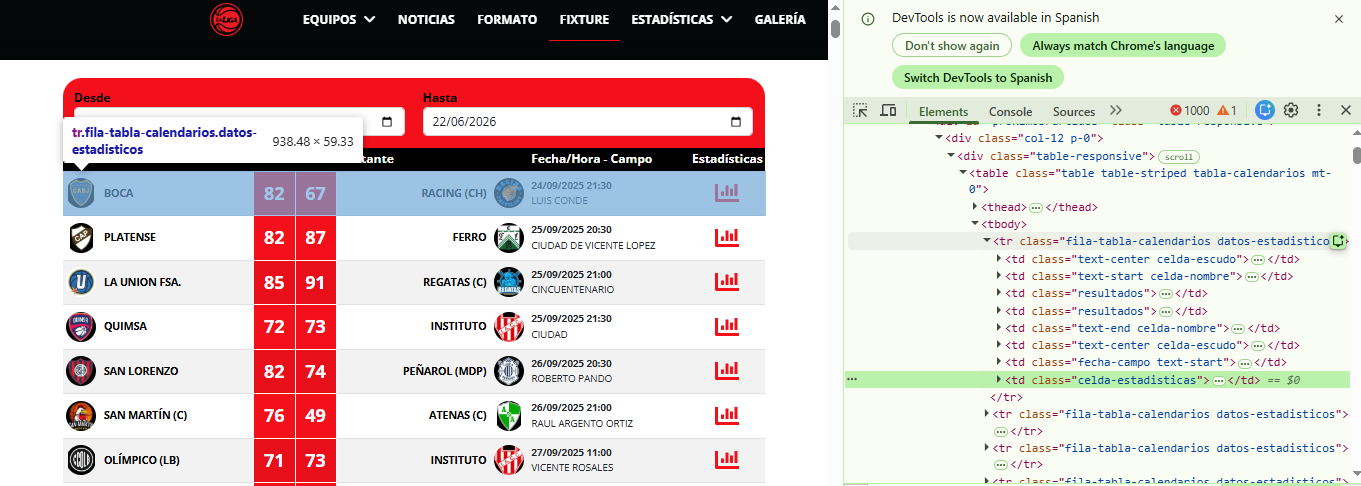
\includegraphics[width=1\linewidth]{img/Captura DOM} 

}

\caption{Inspección de la página web.}\label{fig:unnamed-chunk-4}
\end{figure}

A partir de dicho archivo de texto, se utiliza la librería
\texttt{BeautifulSoup} de Python para recorrer la estructura del DOM,
identificando previamente los elementos que contienen los enlaces de
cada partido. Se observa en la Figura 2 que la información de cada
partido se encuentra dentro de las clases ``fila-tabla-calendarios
datos-estadisticos'', por lo cual se recorren estas clases obteniendo
los respectivos enlaces a las páginas de estadísticas de cada partido,
los nombres de los equipos participantes y el resultado del encuentro,
para cada uno de los 378 partidos disputados en la temporada regular.
Obteniendo finalmente un diccionario que contenga toda esta información.

Dicho diccionario constituyó el insumo básico para el proceso posterior
de scraping masivo, sobre los cuales se iterará para obtener así la
información correspondiente a cada una de las acciones registradas en
cada partido. Esta estrategia permitió, además, asegurar la
reproducibilidad del proceso, ya que el listado de partidos es eliminado
de la página web una vez terminada la temporada, quedando fijado y
documentado de manera explícita para su uso, en caso de ser requerido.

\subsubsection{\texorpdfstring{Base de datos
\emph{play-by-play}}{Base de datos play-by-play}}\label{base-de-datos-play-by-play}

Una vez obtenido el listado completo de enlaces correspondientes a cada
uno de los partidos en el período de estudio, se procedió a la
extracción del registro de acciones del partido (\emph{play-by-play}).
Para esto, se accedió individualmente a la página de estadísticas de
cada encuentro, particularmente a la pestaña denominada ``en vivo'',
donde se presenta el detalle secuencial de los eventos.

Como se observa en la Figura 3, esta sección del sitio web contiene una
tabla que se genera dinámicamente y que registra, en orden cronológico,
todas las acciones ocurridas durante el partido.

\begin{figure}[H]

{\centering \includegraphics[width=0.7\linewidth]{img/imagen play by play_1} 

}

\caption{Pestaña en vivo dentro de la página web de estadísticas de un partido}\label{fig:unnamed-chunk-5}
\end{figure}

En dicha tabla, cada acción del partido se encuentra representada como
un elemento que incluye información textual sobre el tipo de acción (por
ejemplo, lanzamiento convertido, falta, pérdida, etc), el jugador que
realiza dicha acción, el cuarto de juego, el tiempo restante en el
cuarto y , en caso de ser una acción donde se generan puntos, el
marcador parcial en ese momento del partido. Esta información fue
sistemáticamente extraída y almacenada en una estructura tabular,
conservando el orden temporal de las acciones.

Este procedimiento se aplicó de forma idéntica a todos los partidos de
la temporada analizada, utilizando como insumo los enlaces previamente
identificados. Finalmente, los registros de acciones obtenidos para cada
encuentro fueron concatenados en una única base de datos de
\emph{play-by-play}, incorporando un identificador de partido que
permite distinguir y vincular las acciones correspondientes a cada
juego. Asimismo, a partir de esta clave única asociada al encuentro (por
ejemplo, GIMNASIA (CR) vs REGATAS (C) (03/05/2025 20:30)), fue posible
identificar e incorporar a la base el equipo local y visitante
correspondiente a cada partido. Esta información resultó útil en etapas
posteriores del procesamiento donde al conocer el equipo asociado a cada
acción, puede inferirse la condición del mismo (local o visitante).

Es importante destacar que el \emph{dataset} resultante constituye una
secuencia detallada de eventos, pero en su forma original no incluye una
identificación explícita del equipo asociado a cada acción, lo cual
resulta indispensable a la hora de realizar los análisis posteriores.

\subsubsection{Tabla de
jugadores-equipos}\label{tabla-de-jugadores-equipos}

Para resolver este problema, se obtuvo dicha información a partir de los
datos provenientes del \emph{Box Score}, localizados en la pestaña
``Estadísticas'' de la página web del partido (Figura 4). Aquí
encontraremos información referida a cada uno de los jugadores anotados
en la planilla de ambos equipos.

\begin{figure}[H]

{\centering \includegraphics[width=0.7\linewidth]{img/imagen box score} 

}

\caption{Ejemplo del Box Score de un partido}\label{fig:unnamed-chunk-7}
\end{figure}

En esta pestaña, la información se organiza en dos tablas con
estadísticas individuales de los jugadores, una correspondiente al
equipo local y otra al equipo visitante, las cuales aparecen en el mismo
orden en que se muestran los nombres de los equipos en la interfaz del
sitio web. A partir de esta estructura, se extrajo para cada jugador su
nombre completo, el equipo al que pertenece y la cantidad de minutos
disputados en dicho partido, generándose así una tabla de
correspondencia jugador--equipo.

Esta tabla constituye un diccionario que permite asociar a cada jugador
con su respectivo equipo, y es utilizada posteriormente como insumo para
realizar dicha correspondencia en cada acción de la base
\emph{play-by-play}. A su vez, mediante la adición de la cantidad de
minutos en el partido se realiza un filtrado de jugadores que hayan
participado menos de cierto umbral requerido de tiempo durante la
temporada, cuestión fundamental a tratar posteriormente en este trabajo.

\subsection{Preprocesamiento de los
datos}\label{preprocesamiento-de-los-datos}

\subsubsection{\texorpdfstring{Integración del \emph{box score} con el
\emph{play-by-play}}{Integración del box score con el play-by-play}}\label{integraciuxf3n-del-box-score-con-el-play-by-play}

Una vez construida la tabla jugadores-equipos, se procedió a integrar
dicha información con la base de datos \emph{play-by-play}. Para ello,
los nombres de los jugadores fueron previamente normalizados con el
objetivo de reducir posibles inconsistencias de formato (espacios
adicionales, diferencias menores de escritura), y luego se utilizó la
correspondencia jugador--equipo para asignar a cada acción del
\emph{play-by-play} el equipo del jugador involucrado.

De este modo, cada acción queda asociada explícitamente a uno de los dos
equipos del partido, aun cuando dicha información no se encuentre
disponible de forma directa en el registro original del
\emph{play-by-play}. Este procedimiento permite identificar qué
jugadores estarán en cancha para cada uno de los equipos, permitiendo
construir los quintetos en cada momento del partido.

\subsubsection{Identificación de los quintetos en cancha al momento de
la
acción}\label{identificaciuxf3n-de-los-quintetos-en-cancha-al-momento-de-la-acciuxf3n}

A partir de la nueva tabla generada, se procedió a construir la
presencia de los jugadores en cancha a lo largo del partido. Para ello,
se identificaron las acciones asociadas a sustituciones, distinguiendo
entre entradas (acción = ENTRA A PISTA) y salidas de jugadores (acción =
ABANDONA LA PISTA), tal como se observa en la Figura 5.

\begin{figure}[H]

{\centering \includegraphics[width=0.5\linewidth]{img/imagen sustitucion} 

}

\caption{Ejemplo de secuencia de acciones con sustitución}\label{fig:unnamed-chunk-8}
\end{figure}

\newpage

El conjunto de jugadores en cancha se actualiza a medida que se recorren
las acciones del partido, reiniciándose al comienzo de cada cuarto. De
este modo, para cada instante del juego se obtiene el conjunto de
jugadores activos en cancha.

Utilizando la tabla jugadores-equipos construida previamente, cada
jugador en cancha fue asignado al equipo local o visitante, permitiendo
reconstruir los quintetos de ambos equipos en cada acción del partido.
Este paso resulta esencial para caracterizar el contexto en el que
ocurre cada acción, ya que al conocer el equipo al que pertenece el
jugador que realiza la acción podemos inferir simultáneamente los
jugadores ofensivos y defensivos presentes en cancha en cada momento.

Una vez reconstruidos los quintetos en cancha para cada acción, se
incorporó un control de consistencia basado en la cantidad total de
jugadores activos. Dado que una situación de juego regular involucra
diez jugadores (cinco por equipo), se podrán identificar aquellas
acciones en las que la cantidad total de jugadores en cancha fuera
superior o inferior a dicho umbral.

\subsubsection{Detección de errores: Carga de los
datos}\label{detecciuxf3n-de-errores-carga-de-los-datos}

Un factor importante a tener en cuenta es que los datos que se
encuentran en el \emph{play-by-play} son cargados de manera manual por
las mesas de control a medida que se desarrolla el partido. Esta tarea
se realiza en el contexto altamente dinámico de un partido, donde las
acciones se suceden con rapidez, lo que puede dar lugar a ciertos
errores en la registración de eventos. En consecuencia, el conjunto de
datos original puede contener inconsistencias que deben ser
identificadas y corregidas antes de su utilización en este trabajo.

Para intentar detectar posibles errores en la conformación de los
quintetos en cancha, se construyó , tal como se menciono anteriormente,
una variable que contabiliza la cantidad de jugadores presentes en cada
quinteto en cada una de las acciones del partido. Dicha variable debería
contabilizar un valor menor a cinco para ambos equipos en todas las
acciones registradas.

De esta manera se detectó un caso puntual en el partido de ZARATE BASKET
vs ATENAS (C), donde el quinteto local registraba 6 jugadores en cancha.
Esta inconsistencia se observó desde el inicio del segundo cuarto (con
10:00 minutos restantes) hasta el minuto 4:42 del mismo período.

Para subsanar este inconveniente, se realizó una revisión manual del
\emph{play-by-play} original disponible en la página web y se pudo
identificar que al comienzo del segundo cuarto se había registrado
incorrectamente el ingreso de seis jugadores en lugar de cinco, lo cual
constituye un error atribuible a la mesa de control. Una vez
identificada esta problemática, se reviso el contexto de las siguientes
jugadas y pudo determinarse que el jugador MERCHANT, EDGAR HENRY no se
encontraba realmente en cancha durante ese tramo del partido.

En consecuencia, se procedió a corregir el error eliminando al jugador
mencionado de la variable correspondiente al quinteto local en las
acciones afectadas, así como ajustando el conteo de jugadores en cancha.
De esta manera, se restauró la consistencia lógica de los quintetos y se
garantizó la validez de la información utilizada en las etapas
posteriores del análisis.

\subsection{\texorpdfstring{Generación de la base de datos
\emph{poss-by-poss}}{Generación de la base de datos poss-by-poss}}\label{generaciuxf3n-de-la-base-de-datos-poss-by-poss}

Como resultado de las etapas anteriores, pudimos obtener una base de
datos unificada donde cada fila se corresponde con cada una de las
jugadas o acciones que suceden dentro del partido, incluyendo
información relevante para este trabajo como lo es el marcador del
partido al momento de la acción, la composición de los quintetos en
cancha y la condición de local o visitante. Sin embargo, para poder
aplicar los modelos estadísticos mencionados, resulta necesario agrupar
estas acciones en \textbf{posesiones}, entendidas como el conjunto de
acciones ocurridas antes de que cambie el control de la pelota.

Para llevar a cabo este proceso fue necesario definir una metodología
adecuada que permita diferenciar qué acciones pertenecían a una misma
posesión, y en qué momento comenzaba una distinta.

\subsubsection{Eliminación de acciones no relevantes para la
posesión}\label{eliminaciuxf3n-de-acciones-no-relevantes-para-la-posesiuxf3n}

Este procedimiento no pudo realizarse de manera directa, ya que, a pesar
de contar con la información secuencial sobre el que equipo realizaba
cada acción, no todo cambio en el equipo asociado a una acción implica
necesariamente un cambio de posesión del balón. Existen situaciones en
las que se registran acciones del equipo defensor dentro de una posesión
del equipo atacante. A los cuales se ha decidido por llamar como
``acciones intrusas''. Un ejemplo de la contabilización correcta e
incorrecta de las posesiones a partir de la secuencia de acciones se
presenta en la Figura 6.

\begin{figure}[H]

{\centering \includegraphics[width=0.7\linewidth]{img/acciones intrusas} 

}

\caption{Comparación entre distintas formas de contabilizar las posesiones}\label{fig:unnamed-chunk-9}
\end{figure}

Luego de hacer una revisión manual en un conjunto limitado de partidos,
se llegó a la definición de que el conjunto de acciones presentes en el
Cuadro 1 suelen ser siempre acciones intrusas o nunca resultan
informativas para la delimitación de las posesiones. En consecuencia se
ha decidido eliminar las filas en las que ocurren estas acciones en la
base de datos.

Estas acciones son:

\begin{table}[!h]
\centering
\caption{\label{tab:unnamed-chunk-10}Acciones eliminadas por no ser informativas para la delimitación de las posesiones}
\centering
\fontsize{9}{11}\selectfont
\begin{tabular}[t]{>{\raggedleft\arraybackslash}p{1.5cm}>{\raggedright\arraybackslash}p{12cm}}
\toprule
N° & Acción\\
\midrule
\textbf{1} & ENTRA A PISTA\\
\textbf{2} & INICIO DEL PERIODO\\
\textbf{3} & FINAL DEL PERIODO\\
\textbf{4} & ABANDONA LA PISTA\\
\textbf{5} & TAPON REALIZADO\\
\addlinespace
\textbf{6} & TECNICA\\
\textbf{7} & TECNICA BANQUILLO (C)\\
\textbf{8} & TECNICA BANQUILLO (B)\\
\textbf{9} & TECNICA DESCALIFICANTE\\
\textbf{10} & TECNICA DESCALIFICANTE ACOMPAÑANTE NO PARTICIPA\\
\addlinespace
\textbf{11} & TECNICA-E (ALINEACIÓN ILEGAL)\\
\textbf{12} & TIEMPO MUERTO SOLICITADO\\
\textbf{13} & ANTIDEPORTIVA\\
\bottomrule
\end{tabular}
\end{table}

\subsubsection{Manejo de otro tipo de acciones
particulares}\label{manejo-de-otro-tipo-de-acciones-particulares}

\begin{enumerate}
\def\labelenumi{\arabic{enumi})}
\tightlist
\item
  Tratamiento de la flecha de alternancia
\end{enumerate}

En el básquetbol bajo reglamento FIBA, la flecha de alternancia
determina la posesión del balón en los inicios de cuarto o en
situaciones de salto entre dos. Cuando este evento aparece registrado en
el \emph{play-by-play}, el equipo que obtiene la posesión es el opuesto
al que figura inicialmente asociado a la acción.

Para corregir este comportamiento, se implementó una regla que invierte
el equipo asignado a la acción en presencia de una flecha de
alternancia, garantizando la correcta identificación del equipo en
control del balón.

\begin{enumerate}
\def\labelenumi{\arabic{enumi})}
\setcounter{enumi}{1}
\tightlist
\item
  Eliminación de rebotes defensivos al final de cada cuarto
\end{enumerate}

Se detectó que, en algunos casos, el \emph{play-by-play} registra un
rebote defensivo como última acción de un cuarto. Ya que esta situación
sucede quedando unos pocos segundos para terminar el cuarto, no debe ser
contabilizada como una posesión real, y para evitar dichas situaciones
se eliminó dichas acciones de la base de datos.

\begin{enumerate}
\def\labelenumi{\arabic{enumi})}
\setcounter{enumi}{2}
\tightlist
\item
  Reglas específicas para el tratamiento de faltas ofensivas
\end{enumerate}

Las faltas ofensivas representan un caso particular dentro del
\emph{play-by-play}, ya que no son diferenciadas de las faltas
defensivas en la descripción de la acción, y tienen una diferencia
fundamental a la hora de definir las posesiones. Por un lado, las faltas
defensivas corresponden a una ``acción intrusa'' y deben ser eliminadas
de la base, mientras que las faltas ofensivas siempre implican un cambio
inmediato de posesión y, en ocasiones, pueden ser la única acción que
realice un equipo dentro de una posesión, como se observa en la Figura
7. Por lo que en esos casos puntuales dicha acción debe conservarse.

En consecuencia, se desarrolló un conjunto de reglas basadas en el
contexto de la acción previa para decidir si una falta debe ser
conservada o eliminada del registro. Particularmente, se definió que:
una falta debe conservarse si el equipo que la comete es distinto al
equipo que realizó la acción inmediata anterior, siempre que dicha
acción previa sea:

\begin{enumerate}
\def\labelenumi{\arabic{enumi})}
\tightlist
\item
  un lanzamiento fallido.
\item
  una pérdida de balón.
\item
  Una anotación con una separación temporal suficiente que indique el
  transcurso de una nueva posesión.
\end{enumerate}

Todas las faltas que no cumplían esta condición fueron eliminadas para
evitar errores en el conteo de posesiones.

\begin{figure}[H]

{\centering \includegraphics[width=0.7\linewidth]{img/falta ofensiva} 

}

\caption{Ejemplo de falta ofensiva en una secuencia de acciones}\label{fig:unnamed-chunk-11}
\end{figure}

\subsubsection{Identificación de la finalización de las
posesiones}\label{identificaciuxf3n-de-la-finalizaciuxf3n-de-las-posesiones}

Una vez realizada está tarea de preprocesamiento anteriormente
mencionada, se incorporó un identificador preliminar de posesión, basado
en dos criterios fundamentales: el cambio de equipo en control del balón
y el cambio de cuarto. De manera que cada vez que ocurre alguno de estos
eventos, se identifica como el inicio de una nueva posesión. Esto se
encuentra ejemplificado en el Cuadro 2.

\begin{table}[!h]
\centering
\caption{\label{tab:unnamed-chunk-12}Ejemplo de secuencia de acciones diferenciando cada posesión}
\centering
\resizebox{\ifdim\width>\linewidth\linewidth\else\width\fi}{!}{
\fontsize{9}{11}\selectfont
\begin{tabular}[t]{rlllllr}
\toprule
Cuarto & Tiempo & Acción & Jugador & Equipo & ... & Posesión\\
\midrule
1 & 00:08:54 & TIRO DE 3 FALLADO & STENTA, NICOLAS & BOCA &  & 4\\
1 & 00:09:12 & REBOTE DEFENSIVO \#11 & VILDOZA, JOSE IGNACIO & BOCA &  & 4\\
1 & 00:09:13 & TIRO DE 3 FALLADO & BUEMO, CARLOS EMANUEL & ATENAS &  & 3\\
1 & 00:09:18 & FALTA RECIBIDA & BUENDIA, CARLOS MANUEL & ATENAS &  & 3\\
1 & 00:09:31 & ASISTENCIA & VILDOZA, JOSE IGNACIO & BOCA &  & 2\\
\addlinespace
1 & 00:09:32 & TRIPLE & PIÑERO, FACUNDO & BOCA &  & 2\\
1 & 00:09:42 & REBOTE DEFENSIVO \#11 & VILDOZA, JOSE IGNACIO & BOCA &  & 2\\
1 & 00:09:43 & TIRO DE 2 FALLADO & OBERTO, JUAN CRUZ MATEO & ATENAS &  & 1\\
\bottomrule
\end{tabular}}
\end{table}

De este modo, se seleccionaron las filas correspondientes a los eventos
finales de cada posesión, descartando las acciones intermedias que no
determinan su conclusión.

\subsubsection{Cálculo de puntos por
posesión}\label{cuxe1lculo-de-puntos-por-posesiuxf3n}

Para obtener la cantidad de puntos obtenidos en cada posesión, se
calculó la diferencia entre el puntaje acumulado del equipo atacante al
final de la posesión y el puntaje acumulado registrado al cierre de la
posesión inmediatamente anterior. De esta manera, cada posesión queda
caracterizada por una variable discreta que representa su resultado
ofensivo en términos de puntos anotados. Tal como se presenta en el
Cuadro 3.

\begin{table}[!h]
\centering
\caption{\label{tab:unnamed-chunk-13}Ejemplo de estructura con una fila por posesión}
\centering
\resizebox{\ifdim\width>\linewidth\linewidth\else\width\fi}{!}{
\fontsize{9}{11}\selectfont
\begin{tabular}[t]{rlllllrr}
\toprule
Cuarto & Tiempo & Acción & Jugador & Equipo & ... & Posesión & Puntos\\
\midrule
1 & 00:08:54 & TIRO DE 3 FALLADO & STENTA, NICOLAS & BOCA &  & 4 & 0\\
1 & 00:09:13 & TIRO DE 3 FALLADO & BUEMO, CARLOS EMANUEL & ATENAS &  & 3 & 0\\
1 & 00:09:31 & ASISTENCIA & VILDOZA, JOSE IGNACIO & BOCA &  & 2 & 3\\
1 & 00:09:43 & TIRO DE 2 FALLADO & OBERTO, JUAN CRUZ MATEO & ATENAS &  & 1 & 0\\
\bottomrule
\end{tabular}}
\end{table}

\subsubsection{Identificación de jugadores ofensivos y defensivos en
cancha}\label{identificaciuxf3n-de-jugadores-ofensivos-y-defensivos-en-cancha}

Con el objetivo de poder distinguir la participación individual de los
jugadores en cada posesión, se utilizó la información de los quintetos
en cancha previamente reconstruidos durante el preprocesamiento. Para
cada posesión se identificaron los cinco jugadores del equipo atacante y
los cinco jugadores del equipo defensor.

A partir de esta información se construyó una representación matricial
de jugadores por posesión, donde cada jugador de la temporada cuenta con
dos variables indicadora. En la cual, la primer variable dummy asigna a
cada jugador un 1 si el jugador forma parte del quinteto ofensivo y 0 en
caso contratrio; mientras que la segunda variable dummy asigna un -1 si
el jugador forma parte del quinteto defensivo, y 0 en otro caso. Este
esquema permite modelar de manera explícita la contribución ofensiva y
defensiva de manera independiente/separada para cada uno de los
jugadores que han participado en al menos un partido dentro de la
temporada en estudio.

\subsection{\texorpdfstring{Base de datos final:
\emph{poss-by-poss}}{Base de datos final: poss-by-poss}}\label{base-de-datos-final-poss-by-poss}

A través de este proceso, se generó una base de datos que permitirá
modelar la cantidad de puntos por posesión teniendo en cuenta los
jugadores presentes en cancha, dicha base cuenta con la información
correspondiente a 58.625 posesiones, asociadas a 378 partidos disputados
en la temporada en estudio.

Las variables presentes son las siguientes:

\texttt{puntos} = Cantidad de puntos en la posesión.

\texttt{cuarto} = Cuarto en el que se desarrollo la posesión.

\texttt{tiempo} = Tiempo restante del cuarto en el momento que finaliza
la acción.

\texttt{equipo} = Nombre del equipo que está atacando en la posesión.

\texttt{condicion} = Condición de localia del equipo que está atacando
en la posesión.

\section{Metodología}\label{metodologuxeda}

En base a los objetivos planteados en esta tesina de grado, se
compararán resultados provistos por modelos con distintas
características, con el fin de poder sintetizar la contribución ofensiva
y defensiva de los jugadores de manera adecuada. Para poder identificar
que modelo es el que brinda mejores resultados, también se definirá un
procedimiento adecuado para evaluarlos.

Los distintos modelos utilizados, las formas de estimar los parámetros y
los métodos de comparación de modelos se definen a continuación.

\subsection{Modelos propuestos}\label{modelos-propuestos}

\subsubsection{Modelo de regresión lineal
múltiple}\label{modelo-de-regresiuxf3n-lineal-muxfaltiple}

Los modelos más comunmente utilizados en la literatura relevante sobre
RAPMs son los modelos de regresión lineal múltiple, los cuales van a
modelar el comportamiento de la variable respuesta \emph{Puntos en la
posesión i} (\(y_i\)) en función de P = 2K variables explicativas
dicotómicas, correspondientes a las apariciones ofensivas y defensivas
de K jugadores.

El componente aleatorio supone que las respuestas \(y_i\) tienen
variancias constantes \(\sigma^2\). De esta manera tenemos que,

\[\begin{cases}
y_i \sim N(\mu_i  , \sigma^2) \\
\mu_i = \beta_0 + \sum_{j=1}^{K} \beta^o_j x^o_{ji} + \sum_{j=1}^{K} \beta^d_j x^d_{ji}
\end{cases} \]

para \(i = 1,...,n\);

Donde:

\(n\): es el número total de posesiones en nuestro dataset, \(K\): es el
número total de jugadores en consideración, \(y_i\): es el número de
puntos realizados en la posesión \(i\) (los puntos en una posesión
pueden variar de 0 a 7, siendo los casos en que se anotan 6 o 7 puntos,
jugadas extremadamente atípicas), \(\mu_i\): es la cantidad esperada de
puntos anotados en la posesión i, \(x^o_{ik}\): indicadora ofensiva del
jugador k en la posesión i (\(1\) si el jugador \(k\) estaba jugando en
ataque en la posesión \(i\), \(0\) en otro caso), \(x^d_{ik}\):
indicadora defensiva del jugador k en la posesión i (\(-1\) si el
jugador \(k\) estaba jugando en defensa en la posesión \(i\), \(0\) en
otro caso), \(\beta_0\): Intercepto del modelo (usualmente representa al
jugador de referencia, definido como aquel con coeficientes RAPM iguales
o cercanos a cero), \(\beta^o_k\): coeficiente ofensivo del jugador k
(\(ORAPM\)), \(\beta^d_k\): coeficiente defensivo del jugador k
(\(DRAPM\)).

Como \(\hat{\beta}_j\) es una combinacion lineal de \(y_j\) , entonces
la distribución de estos parámetros es conocida. Tenemos que:

\[\hat{\beta}_j \sim N(\beta_j, var[\hat{\beta_j}])\]

Este modelo es de sencilla aplicación y ha sido ampliamente utilizado
por distintos analistas que trabajan con este tipo de métricas. Sin
embargo, la variable respuesta en este caso es discreta, tomando valores
enteros entre 0 y 6, lo que sugiere que el supuesto de normalidad del
modelo de regresión lineal múltiple no resulta apropiado para
representar adecuadamente la naturaleza de la variable de interés.

\paragraph{Interpretación de los
coeficientes}\label{interpretaciuxf3n-de-los-coeficientes}

\ldots{}

\subsubsection{Modelo logístico
multinomial}\label{modelo-loguxedstico-multinomial}

En consecuencia a lo comentado anteriormente, podría ser más razonable
emplear un modelo que contemple la distribución discreta de los datos.
Por lo que se procede a la implementación de una regresión logística
multinomial para modelar el resultado en puntos de cada posesión.

Recordando que \(y_i\) es igual a la cantidad de puntos en una posesión,
nuestra nueva variable respuesta resulta:

\[
y^M_i =
\begin{cases}
y_i, & \text{para } y_i \in \{0, 1, 2\} \\
3, & \text{para } y_i \geq 3
\end{cases}
\] Donde, \(y^M_i \sim Multinomial(n, \boldsymbol{\pi_i})\) con
\(\boldsymbol{\pi_i} = (\pi_{i0},\pi_{i1},\pi_{i2},\pi_{i3})\) y
\(\sum_{c=0}^3 \pi_{ic}=1\).

Resultando \(\pi_{i0},\pi_{i1},\pi_{i2}\) y \(\pi_{i3}\) las
probabilidades respectivas de no anotar, de anotar 1 punto, de anotar 2
puntos y de anotar 3 puntos o más en la posesión \(i\).

Luego construimos el modelo logístico multinomial con categoría de
referencia, eligiendo como categoría de referencia a \(0\) puntos
anotados:

\[logit(\pi_{ic}) = log(\frac{\pi_{ic}}{\pi_{i0}})=\beta_{0c} + \sum_{j=1}^{K} \beta^o_{jc} x^o_{ji} + \sum_{j=1}^{K} \beta^d_{jc} x^d_{ji}\quad \text{con } c= \{1,2, 3\} \]

Dicho modelo describe el efecto de los jugadores en cada uno de los
\(c-1 =3\) logits, es decir, va a permitir calcular el aporte ofensivo y
defensivo del jugador para cada tipo de anotación.

Las probabilidades multinomiales se obtienen mediante las siguientes
ecuaciones:

\[\pi_{ic}=\frac{exp(\boldsymbol{x}_i^T\boldsymbol{\beta}_i)}{1+\sum_{c=1}^3exp(\boldsymbol{x}_i^T\boldsymbol{\beta}_i)} \]

\paragraph{Interpretación de los
coeficientes}\label{interpretaciuxf3n-de-los-coeficientes-1}

\ldots{}

\subsection{EPTS y wEPTS}\label{epts-y-wepts}

\subsubsection{EPTS}\label{epts}

En el enfoque mencionado anteriormente los coeficientes
\{\(\beta_1^o\),\(\beta_2^o\),\(\beta_3^o\)\} y
\{\(\beta_1^d\),\(\beta_2^d\),\(\beta_3^d\)\} representan las
contribuciones de cada jugador en los distintos tipos de anotación.
Aunque puede resultar interesante y permita realizar distintos análisis,
el objetivo final de este estudio es obtener una métrica que unifique la
contribución ofensiva y defensiva en una única medida general.

Para la contribución ofensiva, esto puede lograrse calculando la
cantidad de puntos esperada en una posesión que anota el equipo de dicho
jugador cuando el está incluido en el quinteto y todos los demás
jugadores en la alineación pertenecen al grupo de referencia (con RAPM
igual a 0).

Para la contribución defensiva de un jugador puede evaluarse mediante la
cantidad esperada de puntos (por posesión) concedidos por el equipo de
dicho jugador cuando él no está en la alineación y todos los demás
jugadores en cancha pertenecen al grupo de referencia.

A esta nueva métrica la denominamos ETPS (\emph{Expected Points per Team
possession with the player Scoring contribution})

\[
EPTS_k^r= E(PTS_i \mid X_{ik}^r \ne 0,\, \boldsymbol{X}_{i/k}^r = 0,\, \boldsymbol{X}_i^{\overline{r}} = 0), \quad r \in \{o, d\}
\]

Estas dos medidas, \(ETPS^o\) y \(ETPS^d\), serán funciones de los
coeficientes ofensivos y defensivos del modelo multinomial ajustado. Se
obtienen mediante:

\[EPTS_k^r= \pi^r_{k1}+2\pi_{k2}^r+3,01\pi_{k3}^r, \quad r \in \{o,d\}\]

Donde \(\pi_{kc}^o\) son las probabilidades estimadas mediante un modelo
de regresión logística multinomial de anotar uno, dos o tres puntos o
más, respectivamente, por posesión del equipo del jugador k cuando él
está incluido en la alineación y todos sus compañeros de equipo en la
alineación y todos los oponentes son jugadores incluidos en el grupo de
referencia (es decir, aquellos con coeficientes de regresión iguales a
cero).

De manera similar, \(\pi_{kc}^d\) son las probabilidades de anotar uno,
dos o tres puntos o más, respectivamente, por posesión por parte del
equipo oponente del jugador k cuando dicho jugador no está incluido en
la alineación, bajo el mismo escenario.

Estas probabilidades vienen dadas por:

\[\pi_{kc}^r=\frac{exp(\mu_{kc}^r)}{1+exp(\mu_{k1}^r)+exp(\mu_{k2}^r)+exp(\mu_{k3}^r)} \quad \text{con } \mu_{kc}^r=\beta_{0c}+\beta_{kc}^r\]

\subsubsection{wEPTS}\label{wepts}

Una versión mejorada y ponderada de los EPTS se calcula en
\emph{Damoulaki et.al} (2025), la cual tiene en cuenta la participación
del jugador a lo largo de la temporada. En la cual la métrica
anteriormente presentada se pondera según la proporción de posesiones en
las que el jugador de interés estuvo en cancha. Por lo tanto, el EPTS
ponderado (wEPTS) se define como:

\[
\begin{aligned}
wEPTS_k^{r} &= E(Pts_i \mid \boldsymbol{X}_{i\setminus{k}}^{r} = \boldsymbol{0},\, \boldsymbol{X}_i^{\,\bar{r}} = \boldsymbol{0},\, T_i = t_k) \\[6pt]
&= P(X_{ik}^{r} \ne 0 \mid T_i = t_k) \, E(Pts_i \mid X_{ik}^{r} \ne 0,\boldsymbol{X}_{i\setminus{k}}^{r} = \boldsymbol{0},\, \boldsymbol{X}_i^{\,\bar{r}} = \boldsymbol{0}) \\[6pt]
&\quad + P(X_{ik}^{r} = 0 \mid T_i = t_k) \, E(Pts_i \mid X_{ik}^{r} \ne 0,\boldsymbol{X}_{i\setminus{k}}^{r} = \boldsymbol{0},\, \boldsymbol{X}_i^{\,\bar{r}} = \boldsymbol{0}) \\[6pt]
&= W_k^{r} \, EPTS_k^{r} + (1 - W_k^{r}) \, EPTS_0
\end{aligned}
\]

donde \(r \in \{o, d\}\). Además, el peso \(W_k^{r}\) se estima como:

\[
\hat{W}_k^{r} =
\frac{n_k^{r}}{n_{t_k}^{r}}
=
\frac{\sum_{i=1}^{n} \mathcal{I}(X_{ik}^{r} \ne 0)}
     {\sum_{i=1}^{n} \mathcal{I}(T_i^{r} = t_k)}.
\] Ahora tenemos que \(\mathcal{I}(A)\) es una variable indicadora que
vale 1 en caso de que A sea verdadero y 0 en caso contrario, \(T_i^k\)
es el equipo en ataque (\(r=o\)) o en defensa (\(r=d\)) en la posesión
i, \(t_k\) es el equipo del jugador \(k\), \(n_k^r\) es el número de
posesiones en las que el jugador \(k\) participó en el quinteto en
ataque o defensa en la temporada y \(n_{t_k}^r\) es el número de
posesiones en las que el equipo del jugador \(k\) está en ataque o
defensa en la temporada.

\subsection{Multicolinealidad}\label{multicolinealidad}

\ldots{}

\subsection{\texorpdfstring{Tratamiento de los jugadores con poco tiempo
de juego (\emph{Low time players -
LTP})}{Tratamiento de los jugadores con poco tiempo de juego (Low time players - LTP)}}\label{tratamiento-de-los-jugadores-con-poco-tiempo-de-juego-low-time-players---ltp}

\ldots{}

\subsection{Estimación de los RAPMs}\label{estimaciuxf3n-de-los-rapms}

\subsubsection{Método de mínimos
cuadrados}\label{muxe9todo-de-muxednimos-cuadrados}

En el modelo de regresión lineal múltiple, vamos a estimar los
parámetros buscando minimizar las diferencias entre las observaciones de
nuestro dataset y las estimaciones del modelo,

Función a minimizar: \(S = \sum_{i=1}^n w_i(y_i-\mu_i)^2\)

Los estimadores de mínimos cuadrados de \(beta_j\) se definen como
aquellos valores de \(beta_j\) que minimizan la suma de cuadrados \(S\),
y se denotan como \(\hat{\beta}_0, \ldots, \hat{\beta}_p\).

Obteniendo de esta manera los siguientes coeficientes estimados:
\(\hat{\beta_j} = \frac{\sum_{i=1}^n w_ix_{ij}^*y_{i}}{\sum_{i=1}^n w_i(x_{ij}^*)^2}\),

para \(j= 0,...,p\), donde \(x_{ij}^*\) da los valores de la j-ésima
variable explicativa \(x_j\) después de haber sido ajustada por todas
las demás variables explicativas \(x_0,...,x_p\) excepto \(x_j\). La
variable explicativa ajustada \(x_{j}^*\) es aquella parte de \(x_j\)
que no puede ser explicada mediante una regresión sobre las otras
variables explicativas (Dunn y Smyth, 2018).

\subsubsection{Método de máxima
verosimilitud}\label{muxe9todo-de-muxe1xima-verosimilitud}

En el modelo logístico multinomial, los parámetros
\(\beta_0, \beta_1, . . ., \beta_p\) se estiman utilizando
simultáneamente las (c-1) ecuaciones logit, de manera que se maximice la
log-verosimilitud:

Función a maximizar:
\(L_m(\boldsymbol{\beta},\boldsymbol{y})=\sum_{i=1}^nw_i\sum_{j=1}^cy_{ij}log(\pi_{ij}),\)

Como esto no tiene una solución cerrada, debe recurrirse a algoritmos
iterativos como \emph{Newthon-Rapshon} o \emph{Fisher-Scoring} para
obtener los resultados.

\subsection{Métodos de
regularización}\label{muxe9todos-de-regularizaciuxf3n}

Como se ha mencionado anteriormente, el modelo planteado presenta
variables predictoras altamente correlacionadas debido a que muchos de
los jugadores comparten gran parte del tiempo en cancha, por lo que el
ajuste con mínimos cuadrados ordinarios o mediante máxima verosimilitud
se torna inestable. Con el objetivo de solucionar este problema se
realizaran estimaciones mediante métodos de regularización (o
\emph{shrinkage}), los cuales agregan un término de penalización a la
función de pérdida para de esta manera controlar la magnitud de los
coeficientes estimados. Esta técnica va a provocar que las estimaciones
sean sesgadas, pero a cambio de una notable reducción en la variancia.

Las técnicas que se utilizarán en esta investigación son las siguientes:

\subsubsection{Regresión Ridge o Regularización
L2}\label{regresiuxf3n-ridge-o-regularizaciuxf3n-l2}

Este método incorpora una penalización cuadrática sobre los coeficientes
del modelo.

Para el \textbf{modelo de regresión lineal múltiple} los coficientes
estimados \(\hat{\boldsymbol{\beta}}\) se obtienen minimizando la
función de perdida (\(S\)) modificada de la siguiente manera:

\[S^*= \sum_{i=1}^n w_i(y_i-\mu_i)^2 + \lambda \sum_{j=1}^p\beta_j^2=S+\lambda \sum_{j=1}^p\beta_j^2\]

Donde \(\lambda \geq 0\) es un \emph{hiperparámetro} que controla la
intensidad de la penalización.

Cuando \(\lambda = 0\) no hay penalización y la estimación será igual a
la obtenida por mínimos cuadrados; y a medida que \(\lambda\) aumenta la
penalización se vuelve más dominante y los coeficientes tienden a 0.
Para encontrar el valor óptimo de \(\lambda\) se utilizarán técnicas de
\textbf{validación cruzada}.

Mientras que en el caso del \textbf{modelo logístico multinomial}, se
agrega un parámetro de penalización a la función de log-verosimilitud,
de manera tal que la log-verosimilitud penalizada a maximizar resulta:

\[L^*_m(\boldsymbol{\beta},\boldsymbol{y})=\sum_{i=1}^nw_i\sum_{j=1}^cy_{ij}log(\pi_{ij}) + \lambda \sum_{j=1}^p\beta_j^2=L_m(\boldsymbol{\beta},\boldsymbol{y}) + \lambda \sum_{j=1}^p\beta_j^2\]
Y el \emph{hiperparámetro} \(\lambda\) se selecciona nuevamente mediante
validación cruzada.

\subsubsection{Lasso o Regularización
L1}\label{lasso-o-regularizaciuxf3n-l1}

A diferencia de la regresión Ridge, en la cual los coeficientes pueden
acercarse a 0 pero nunca llegan exactamente a ese valor, la técnica
Lasso, presentada por Robert Tibshirani (1996), tiende a forzar algunos
parámetros a ser cero, con lo cual también se realiza una selección de
las variables/jugadores más influyentes. La intención de aplicar está
técnica esta basada en que puede ser útil para resolver el problema de
los coeficientes extremos que presentan los jugadores que juegan pocos
minutos. Además esto permite una interpretación más significativa del
intercepto del modelo implementado, ya que ahora representa la
contribución promedio de un jugador de referencia\footnote{Por jugador
  de referencia entendemos a cualquier jugador que pertenece al grupo de
  jugadores con coeficientes iguales a cero.} en cada posesión.

La penalización en este caso se basa en la suma de los valores absolutos
de los coeficientes.

Para el \textbf{modelo de regresión lineal múltiple} resulta:

\[S^*= \sum_{i=1}^n w_i(y_i-\mu_i)^2 + \lambda \sum_{j=1}^p|\beta_j|=S+\lambda \sum_{j=1}^p\ |\beta_j|\]
Para el \textbf{modelo logístico multinomial} resulta:

\[L^*_m(\boldsymbol{\beta},\boldsymbol{y})=\sum_{i=1}^nw_i\sum_{j=1}^cy_{ij}log(\pi_{ij}) + \lambda \sum_{j=1}^p|\beta_j|=L_m(\boldsymbol{\beta},\boldsymbol{y}) + \lambda \sum_{j=1}^p|\beta_j|\]
En este caso valores grandes de \(\lambda\) incrementan la penalización,
llevando a que un mayor número de coeficientes se reduzcan exactamente a
cero.

\subsubsection{Elastic Net}\label{elastic-net}

Cuando existen predictores altamente correlacionados, \textbf{ridge}
reduce la influencia de todos ellos a la vez de forma proporcional,
mientras que \textbf{lasso} tiende a seleccionar uno de ellos, dándole
todo el peso y excluyendo al resto. En presencia de correlaciones
fuertes esta selección puede variar mucho ante pequeñas perturbaciones ,
por lo que las soluciones de lasso pueden ser más inestables.

Para encontrar un equilibrio entre ambos métodos se plantea la
penalización \textbf{elastic net}, introducido por Hui Zou y Trevor
Hastie (2005), la cual combina las penalizaciones L1 (Lasso) y L2
(Ridge).

Para el \textbf{modelo de regresión lineal múltiple} resulta:

\[S^*= \sum_{i=1}^n w_i(y_i-\mu_i)^2 + \lambda [\alpha\sum_{j=1}^p|\beta_j|+\frac{(1-\alpha)}{2}\sum_{j=1}^p\beta_j^2]=S+\lambda \sum_{j=1}^p[\alpha\sum_{j=1}^p|\beta_j|+\frac{(1-\alpha)}{2}\sum_{j=1}^p\beta_j^2]\]

Para el \textbf{modelo logístico multinomial} resulta:

\[L^*_m(\boldsymbol{\beta},\boldsymbol{y})=\sum_{i=1}^nw_i\sum_{j=1}^cy_{ij}log(\pi_{ij}) + \lambda \sum_{j=1}^p[\alpha\sum_{j=1}^p|\beta_j|+\frac{(1-\alpha)}{2}\sum_{j=1}^p\beta_j^2]=L_m(\boldsymbol{\beta},\boldsymbol{y}) + \lambda \sum_{j=1}^p[\alpha\sum_{j=1}^p|\beta_j|+\frac{(1-\alpha)}{2}\sum_{j=1}^p\beta_j^2]\]
Donde, \(\lambda \geq 0\) sigue siendo el parámetro de regularización
que controla la fuerza de la penalización, y se agrega un nuevo
hiperparámetro \(\alpha \in [0,1]\) que controla la combinación entre
lasso y ridge. Si \(\alpha = 1\) se obtiene lasso y si \(\alpha = 0\) se
obtiene ridge.

\subsection{Tuneo de hiperparámetros}\label{tuneo-de-hiperparuxe1metros}

\ldots{}

\subsection{Comparación de modelos}\label{comparaciuxf3n-de-modelos}

Una vez que se obtengan los ratings de jugadores a través de las
distintas técnicas mencionadas, resulta sumamente importante definir un
método para evaluarlos, y de esta manera poder identificar cual es el
que ofrece mejores resultados.

En el ámbito del fútbol el profesor Lars Magnus Hvattum plantea una
solución muy interesante para esta problemática, la cual no parece haber
sido implementada en básquetbol hasta la fecha. En el artículo
\emph{Modelling the financial contribution of soccer players to their
clubs} (Sæbø \& Hvattum, 2019) y en videos de su página de youtube
\href{https://www.youtube.com/@footballplayerratings}{Football Player
Rating}s se definen 2 criterios diferentes para medir los distintos
sistemas de rankings, buscando evaluar la \textbf{consistencia} y la
\textbf{validez} de los mismos.

\subsubsection{Bondad de ajuste}\label{bondad-de-ajuste}

\ldots{}

\subsubsection{Evaluación de la consistencia de los
resultados}\label{evaluaciuxf3n-de-la-consistencia-de-los-resultados}

Según Hvattum, un buen modelo producirá resultados similares
independientemente de que partidos hayan sido incluidos en el dataset.
Bajo este enfoque, si un mismo sistema de rankings brinda estimaciones
de RAPMs similares al ser aplicado a distintas muestras del dataset (de
tamaños similares), entonces dicho modelo será consistente.

Para evaluar esto, se divide el conjunto de datos completo en dos
particiones con cantidades similares de posesiones. Luego, se calculan
los valores de RAPM para cada partición y se estima la correlación de
Pearson entre ambos conjuntos de coeficientes. Cuanto mayor sea este
coeficiente, mayor será la consistencia del modelo.

\begin{figure}
\centering
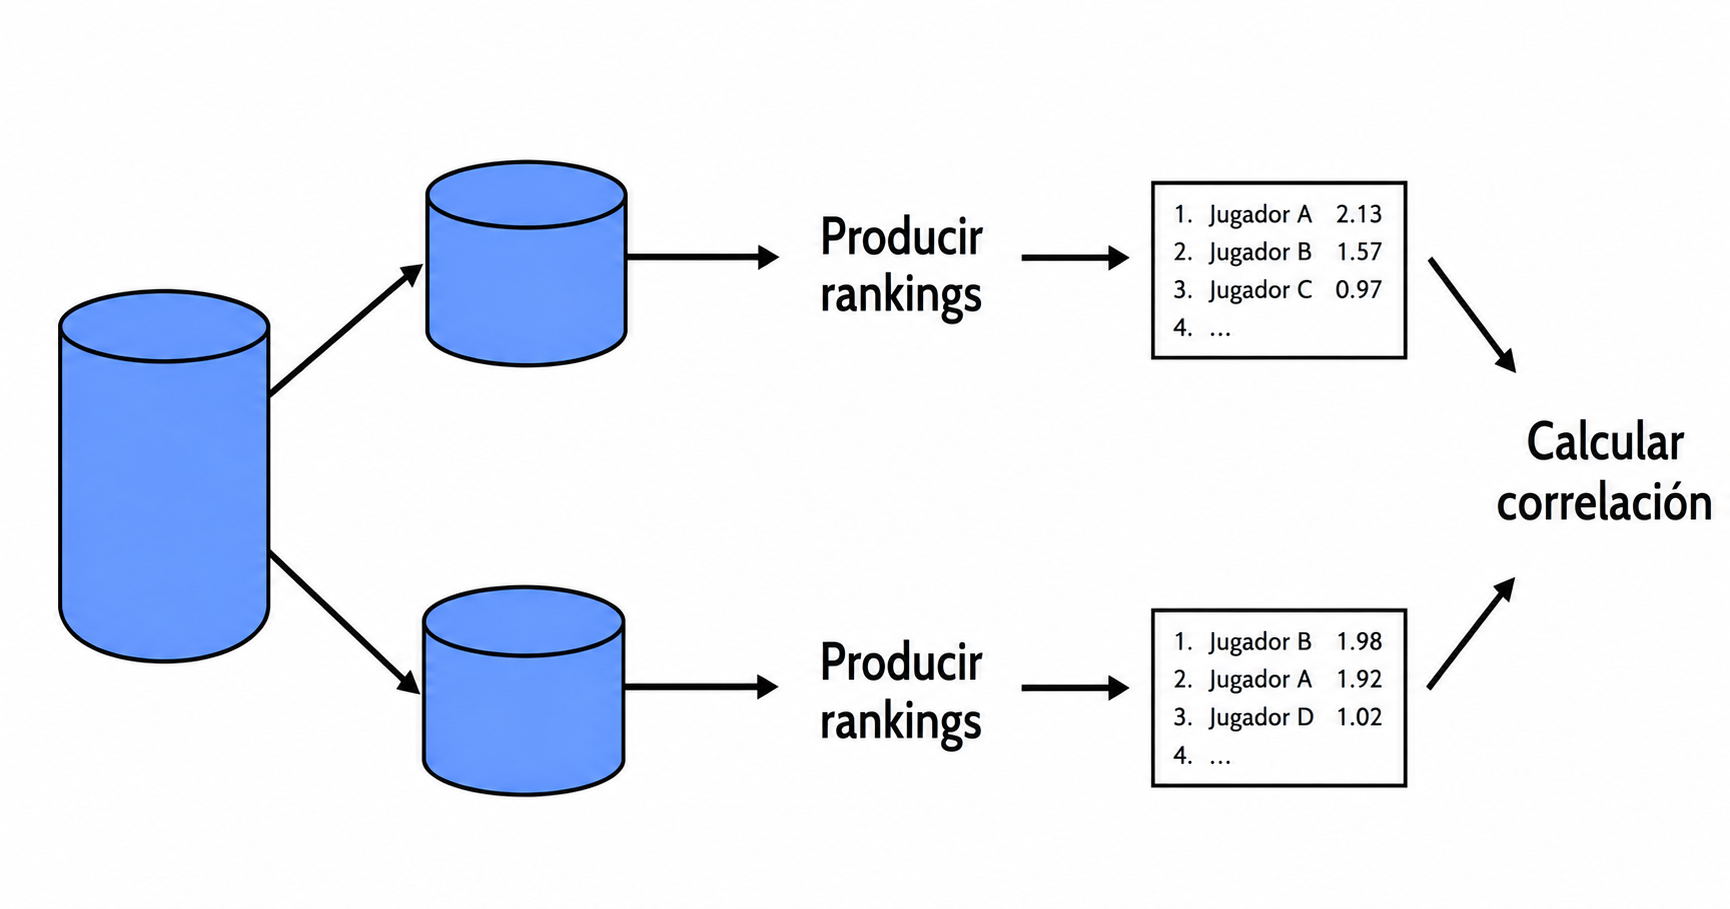
\includegraphics[width=0.8\textwidth,height=\textheight]{img/consistencia-hvattum.PNG}
\caption{Procedimiento para evaluar la consistencia de los modelos
RAPM.\\
Fuente: Hvattum (2023), \emph{How to evaluate football player ratings?}
{[}Video{]}. YouTube.}
\end{figure}

\subsubsection{Criterios de validación
externa}\label{criterios-de-validaciuxf3n-externa}

\ldots{}

\section{Resultados}\label{resultados}

\section{Conclusión}\label{conclusiuxf3n}

\section{Discusión}\label{discusiuxf3n}

Los modelos RAPM utilizados en este trabajo, al igual que la literatura
previa (Rosenbaum, 2004; Sill, 2010; Damoulaki et al., 2025), consideran
cada posesión como una observación independiente. Sin embargo, esta
hipótesis puede resultar discutible, dado que las posesiones
pertenecientes a un mismo partido presentan dependencia temporal
derivada de factores como el ritmo de juego, los ajustes tácticos, la
fatiga y el contexto competitivo. Aunque esta dependencia no
necesariamente sesga las estimaciones de los coeficientes bajo la
hipótesis de exogeneidad de los errores, sí podría afectar su eficiencia
y la correcta cuantificación de la incertidumbre. El desarrollo de
modelos RAPM que incorporen explícitamente la correlación intra-partido
constituye una línea de investigación aún poco explorada.

\href{https://rephip.unr.edu.ar/server/api/core/bitstreams/a4c018fe-9f41-44ee-8d53-d554e3473bb0/content}{INTERPRETACIÓN
Y COMPARACIÓN DE MODELOS DE REGRESIÓN LOGÍSTICA PARA EL ESTUDIO DE LA
DESOCUPACIÓN} (regresión logística con correlación, aplicación de
modelos gee)

comparar lo escrito en este rmd con el que escribi para el anteproyecto,
quizas este era una versión anterior y le faltan correcciones

evaluación de modelos de regresión lineal múltiple

\newpage

\section{Bibliografía}\label{bibliografuxeda}

Agresti, A. (2013). \emph{Categorical Data Analysis} (3rd ed.). Wiley
Series in Probability and Statistics. Wiley, New York.

Damoulaki, A., Ntzoufras, I. \& Pelechrinis, K. (2025). \emph{Lasso
multinomial performance indicators for in-play basketball data.} Comput
Stat 40, 2157--2181.

Dunn, P. K., \& Smyth, G. K. (2018). \emph{Generalized linear models
with examples in R. Springer.}

Hvattum, L. M. (2019). \emph{A comprehensive review of plus--minus
ratings for evaluating individual players in team sports.} International
Journal of Computer Science in Sport, 18, 1--23.

Ilardi, S. (2007). \emph{Adjusted Plus-Minus: An idea whose time has
come.} Blog: 82games. \url{http://www.82games.com/ilardi1.htm}

Ilardi, S., \& Barzilai, A. (2008). \emph{Adjusted Plus-Minus ratings:
New and improved for 2007--2008.} Blog: 82games.
\url{http://www.82games.com/ilardi2.htm}

James, G., Witten, D., Hastie, T., \& Tibshirani, R. (2021). \emph{An
Introduction to Statistical Learning with Applications in R} (ISLR2).

Kubatko, J., Oliver, D., Pelton, K., \& Rosenbaum, D. (2007). \emph{A
starting point for analyzing basketball statistics.} Journal of
Quantitative Analysis in Sports, 3, Article 1.

Rosenbaum, D. (2004). \emph{Measuring how NBA players help their teams
win.} Blog: 82games. \url{http://www.82games.com/comm30.htm}

Sæbø, O., \& Hvattum, L. (2019). \emph{Modelling the financial
contribution of soccer players to their clubs.} Journal of Sports
Analytics, 5, 23--34.

Sill, J. (2010). \emph{Improved NBA adjusted +/-- using regularization
and out-of-sample testing.} Proceedings of the 2010 MIT Sloan Sports
Analytics Conference.

Tibshirani, R. (1996). \emph{Regression shrinkage and selection via the
lasso.} Journal of the Royal Statistical Society: Series B
(Methodological), 58(1), 267--288.

Zou, H., \& Hastie, T. (2005). \emph{Regularization and Variable
Selection via the Elastic Net.} Journal of the Royal Statistical
Society: Series B, 67(2), 301--320.

\end{document}
